
\begin{figure}[ht!]
  \centering
  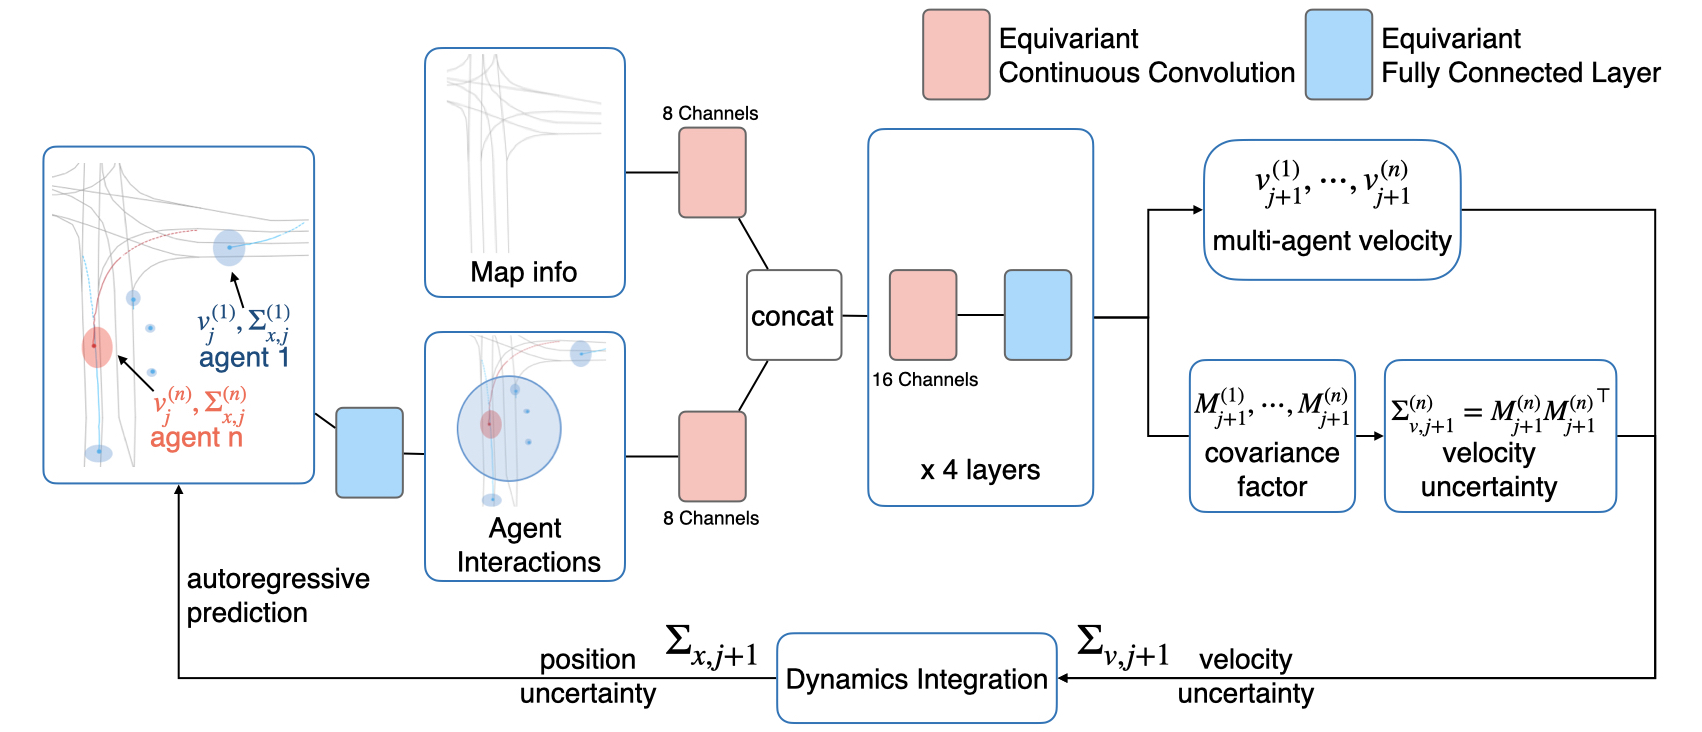
\includegraphics[width=1\linewidth]{equivariance/figs/model2.jpeg}
  %model.pdf
  \caption{Overview of PECCO's model architecture. Agent trajectories consisting of velocities and position uncertainties are encoded along with map information by equivariant continuous convolution and fully connected layers. The model outputs $v_{j+1}$ and $\Sigma_{v,j+1}$ for all agents, which we use to calculate position uncertainty $\Sigma_{x,j+1}$ via dynamics. The model takes in the forecast and predicts autoregressively.} 
  \label{fig:model}
\end{figure}

\subsection{Problem Setup}
 Given  past trajectories of $n$ agents over $t$ time steps $\{x_{j}^{(1)}, x_{j}^{(2)}, \cdots, x_{j}^{(n)} \}_{j=1}^t $, where  ${x}^{(i)}_{j} \in \mathbb{R}^2$ , and the environmental context information $\mathbf{e}$ including marker positions of map lane boundaries, we model the probability distribution of agents' positions over  $k$ future time steps  as $p_\theta( {x}_{t+1:t+k} | {x}_{1:t}, \mathbf{e})$, with ${x}_j = ({x}^{(1)}_{j},\cdots, {x}^{(n)}_{j})$ being the positions of all agents at time step $j$. We introduce  PECCO, a deep learning model that leverages rotational equivariance to produce probabilistic forecasts.


The high-level architecture of our model is illustrated in Figure \ref{fig:model}. PECCO takes as input the positions of all agents ${x}_{1:t}$ in the past, and the covariance matrix $\Sigma_{x,j}$ at time $j$. It outputs the probability distribution of each agents' velocity as a 2-D Gaussian $\T{N}(\mu_{v,j+1}^{(i)}$, $\Sigma_{v,j+1}^{(i)})$ for the next time step. The velocity distribution is then integrated into a position distribution $\mathcal{N}$($\mu_{x, j+1}^{(i)}$, $\Sigma_{x, j+1}^{(i)}$) through dynamics integration. PECCO predicts the future $k$ timesteps autoregressively. The output distributions are guaranteed to be rotational equivariant by our model implementation.

\subsection{Probabilistic Symmetry through Equivariant Neural Networks} 

Rotational equivariance effectively reduces the dimension of the data space by placing different samples in the same equivalence class. This improves data coverage for better probabilistic modeling. 

Intuitively, real-world trajectory dynamics has intrinsic symmetry. That is, if past trajectories and environmental data such as the map is rotated, then the probability of a rotated future trajectory will be equally likely. We can model the probability density function $p_\theta$ as an invariant function of its inputs as in \autoref{eqn:invariant_prob}. Here, each past and future position $x^{(i)}_j \in \mathbb{R}^2$ is transformed according the standard representation $\rho_1$.  
\begin{equation} \label{eqn:invariant_prob}   
    p_\theta( {x}_{t+1:t+k} | {x}_{1:t}, \mathbf{e}) = p_\theta( g{x}_{t+1:t+k} | g{x}_{1:t}, g\mathbf{e}) \quad \forall g\in \SOtwo
\end{equation}


%\rw{explicitly refer to factorization over agents and timesteps?}

In order to implement \autoref{eqn:invariant_prob}, we 
assume future positions  follow a multivariate normal distribution ${x}^{(i)}_{j} \sim N(\mu^{(i)}_{x,j},\Sigma^{(i)}_{x,j})$. This is a common assumption in trajectory forecasting literature \cite{trajpredsurvey} and provides a convenient parametric form for optimization and reasoning. In the following expositions we omit the underscore $x$ for simplicity.

We aim to construct an equivariant neural network $f_\theta$ that outputs the parameters $\mu^{(i)}_{j}$ and $\Sigma^{(i)}_{j}$ autoregressively, taking as input probability distributions over the positions of all agents in the past $k$ time steps
\[
\mu_{j+1},\Sigma_{j+1} = f_\theta(\mu_{j-t+1:j}, \Sigma_{j-t+1:j}, \mathbf{e}). 
\]
where $\mu_{j} = (\mu_{j}^{(1)},\ldots,\mu_{j}^{(n)})$ and $\Sigma_j = (\Sigma_{j}^{(1)},\ldots,\Sigma_{j}^{(n)})$ and $\mathbf{e}$ denotes environmental information.  

In this case, the equivariance of $f_\theta$ leads to the desired invariance of $p_\theta$. This may be seen as a partial evaluation or currying of the conditional probability density function which has the effect of transforming invariance to equivariance. The following proposition relates equivariant networks with probabilistic symmetry. See Appendix \ref{app:equiv_dist} for a proof.
\begin{proposition}[One step equivariance implies $n$-step equivariance] \label{prop:equivtoinvar}
If the one-step probabilistic forecasting model $f_\theta$ is $G$-equivariant, then the probability distribution $p_\theta( x_{t+1:t+k} | x_{1:t}, \mathbf{e})$ is invariant as in \autoref{eqn:invariant_prob}.
\end{proposition}

%\paragraph{Equivariant Conditional Normal Distributions.} 
In order to enforce $\SOtwo$-equivariance for $f_\theta$, the following proposition describes how the mean and covariance matrix for a 2-D  Gaussian  transforms under a rotation of $\mathbb{R}^2$. 

\begin{proposition}[SO(2) equivariance of multivariate Gaussian]  \label{prop:equivnormal}
Given multivariate normal distribution $\mathcal{N}(\mu,\Sigma)$ over $\mathbb{R}^2$ with probability density function $p_{\mu, \Sigma}$ and $g\in \SOtwo$, then $\mathcal{N}(g\mu, g\Sigma g^T)$ is also a multivariate normal distribution and $p_{g\mu, g\Sigma g^T} (v) = p_{\mu, \Sigma} (g^{-1}v)$ for all $v \in \mathbb{R}^2$.
\end{proposition}  

To ensure the covariance matrix of $f_\theta$ is positive-definite and symmetric, i.e. $\Sigma \in \mathrm{PosDefSym}_2(\mathbb{R})$, we make use of the following fact: 

\begin{proposition}[Equivariant maps constructing positive-definite symmetric matrices] \label{prop:pds}
The map
\begin{align}
    \varphi \colon \mathrm{GL}_2(\mathbb{R}) \to \mathrm{PosDefSym}_2(\mathbb{R}) , \quad 
    M \mapsto M M^T \label{eq:phi}
\end{align}
is surjective and equivariant. That is, for $g \in \SOtwo$ we have
\begin{align}
    \varphi(gM) &= g \varphi(M) g^{T} \label{eq:act_on_gl2}. 
\end{align}
Moreover, $\varphi$ admits a one-sided inverse which is also equivariant,
\begin{align}
        \psi \colon \mathrm{PosDefSym}_2(\mathbb{R}) \to \mathrm{GL}_2(\mathbb{R}), \quad    
        \Sigma \mapsto Q \Lambda^{\frac{1}{2}}
\end{align}
where $Q\Lambda Q^T$ is the eigendecomposition of $\Sigma$ and $Q$ is orthogonal. Together, $\varphi (\psi(\Sigma)) = \Sigma$.
\end{proposition}

As a consequence of Proposition \ref{prop:equivnormal} and Proposition \ref{prop:pds}, we can ensure that the predicted distribution transforms correctly under equivariance by (1) predicting an intermediate matrix $M$ for covariance, and (2) constraining $\tilde{f}_\theta$ to be equivariant with respect to the action in \autoref{eq:act_on_gl2}.
\begin{equation} \label{eq:ftheta}
\begin{aligned}    
    \mu_{j+1},M_{j+1} = \tilde{f}_\theta(\mu_{j-k:j}, M_{j-k:j}, \mathbf{e}), \;
    \Sigma_{j+1} = M_{j+1}M_{j+1}^T
\end{aligned}
\end{equation}
In this case, $\SOtwo$ acts by transforming the the columns of $M$ independently as vectors in $\mathbb{R}^2$.  Thus the data $(\mu_j^{(i)},\Sigma_j^{(i)})$ for each agent and time step is comprised of 3 copies of the standard representation $\rho_1$ as defined in Section \ref{subsec:symmetry}.  Given this $\SOtwo$ action, we can enforce $\SOtwo$-equivariance in the neural network $\tilde{f}_\theta$. Implementation details of  of the equivariant layers are provided in Appendix \ref{app:matrix}.


% \begin{proposition}
% If $f_{\theta}$ satisfies then $f_{\theta}$ is equivariant
% \end{proposition}

% [REFERNCE STUFF FROM APPENDIX HERE.  NO PROOFS JUST STATEMENT AND SHORT DESCRIPTION]


%\subsection{Kernel and Weight Sharing Scheme} 

\subsection{Dynamics Integration (dyna)} 
\label{sec:dyn_inte}
Instead of predicting the position directly, PECCO outputs a Gaussian distribution over \emph{velocity} as $\mathcal{N}(\mu_{v,j}, \Sigma_{v,j})$. More specifically, it predicts $(\mu_{v,j}, M_{v,j})$ at each time step and the covariance matrix $\Sigma_{v,j}$ is calculated as in Proposition \ref{prop:pds}. However, we want to obtain the  uncertainty over \textit{position} as $\Sigma_{x,j}$ and perform autoregressive forecasting. We leverage dynamics integration to propagate the uncertainty from velocity to position.


Assuming that all agents in the system can be approximated as linear discrete time dynamics ${x}_{j+1} = {x}_j + \Delta t \cdot  {v}_j $, we can obtain the uncertainty of predicted position $\Sigma_{x, j+1}$ by %  =  \Sigma_{p, t} + \Delta t \cdot \Sigma_{v,t+1}\cdot\Delta t 
\[ 
\Sigma_{x, j+1}
            = \Sigma_{x, j} + (\Delta t)^2 \, \Sigma_{v, j} + 2 \Delta t \cdot \text{cov}(x_j, v_j).
\]
%
We assume that the cross covariance matrix $\mathrm{cov}(x_j, v_j) $ is zero for simplicity 
following previous works \cite{trajectron++}. During training, gradients are calculated after entire trajectory is predicted autoregressively. A consequence of the additive uncertainty setup is that it enforces the uncertainty 
to grow monotonically over time, creating a ``cone of uncertainty".

